\documentclass[a4j]{jarticle}
    \usepackage[dvipdfmx]{graphicx}
    \usepackage[ top=25truemm,bottom=25truemm,left=25truemm,right=25truemm]
    {geometry}
    \usepackage{ascmac}
    \usepackage{array}
    \usepackage{here}
    \usepackage{url}
    \usepackage{listings, jlisting}
    \renewcommand{\lstlistingname}{リスト}
\lstset{language=c,
  basicstyle=\ttfamily\scriptsize,
  commentstyle=\textit,
  classoffset=1,
  keywordstyle=\bfseries,
  frame=tRBl,
  framesep=5pt,
  showstringspaces=false,
  numbers=left,
  stepnumber=1,
  numberstyle=\tiny,
  tabsize=4
}

\makeatletter
\def\@thesis{プログラミング演習 レポート}
\def\id#1{\def\@id{#1}}
\def\department#1{\def\@department{#1}}

\def\@maketitle{
\begin{center}
{\huge \@thesis \par} %修士論文と記載される部分
\vspace{10mm}
{\LARGE\bf \@title \par}% 論文のタイトル部分
\vspace{10mm}
{\Large \@date\par}	% 提出年月日部分
\vspace{20mm}
{\Large \@department \par}	% 所属部分
{\Large 学籍番号 \@id \par}	% 学籍番号部分
\vspace{10mm}
{\Large 氏名 \@author}% 氏名 
\end{center}
\par\vskip 1.5em
}

\title{ミニゲーム}
\date{提出期限 2021年1月18日 17:00}
\department{組番号 408}
\id{17406}
\author{金澤雄大}

    \begin{document}
    \maketitle
    \thispagestyle{empty}
    \clearpage
    \addtocounter{page}{-1}
    \section{目的}
    後期のプログラミング演習で学習した内容の理解度を高めるために,ミニゲームを作成することを目的とする.
    \section{ミニゲームの説明}
    本章では,ゲームの概要,用語,設定,仕様の4つについて述べる.
    \subsection{ゲームの概要}
    ミニゲームとして,「桃太郎電鉄」\cite{mmtt}(以下,桃鉄)をイメージした「ちゃま鉄」を作成した.「ちゃま鉄」は鉄道会社の運営をイメージしたすごろく形式のゲームである.
    本ゲームは,3年決戦で3人でのプレイを想定しており,CPUキャラは存在しない.また桃鉄における「貧乏神」,「すりの銀次」,「臨時収入」を代表とする要素は開発時間の都合上実装していない.
    \subsection{プレイヤーと物件の設定}
    プレイヤーおよび物件の設定について説明する.先述した通り,プレイヤー(社長と呼ぶ)は3人おり,ゲーム内ではターン順に「プレイヤー1社長」,「プレイヤー2社長」,「プレイヤー3社長」と
    呼ばれる仕様になっている.さらに各社長には色の設定が行われている.社長名と色の対応を次に示す.
    \begin{itemize}
        \item プレイヤー1社長 $\cdots$ 青
        \item プレイヤー2社長 $\cdots$ ピンク
        \item プレイヤー3社長 $\cdots$ 黄色
      \end{itemize}
       各社長には「所持金」,「総資産」という2つのパラメータが割り振られている.ゲームスタート時の所持金は1億円,総資産は0円である.所持金は社長が手元に持っているお金のことである.停車する駅には
      「物件」を購入できる「物件駅」というものがあり,この物件を購入することで総資産を増やすことができる.図\ref{bukkenex}に長野駅の物件の例を示す.
      図\ref{bukkenex}には6つの物件がある.物件には「価格」,「収益率」という2つのパラメータがある.例えば「りんごえん」の場合,価格が「600万円」,収益率が「120\%」である.
      価格はその物件を購入するために必要な所持金であり,収益率は決算(後述)で手に入るお金の割合を示している.また,同じ駅の物件を1人の社長がすべて購入すると「独占」という
      状態になる.独占状態になった駅の収益率は2倍になり,決算で2倍の収益が得られる仕様になっている.

      \begin{figure}[H]
        \centering
        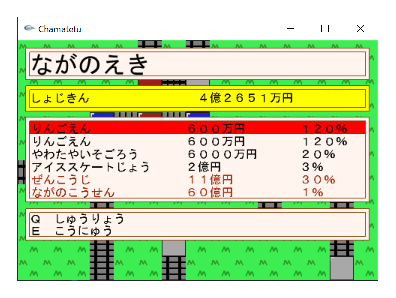
\includegraphics[scale=1.5]{bukkenex.eps}
        \caption{物件の例(長野駅)}
         \label{bukkenex}
        \end{figure}
    
    \subsection{ゲームの進行方法}
    ゲームの進行について説明する.ここではゲームの進行の概要について説明し,実際の画面表示については実装部分と共に述べる.
    図\ref{processgame}にゲーム進行のフローチャートを示す.ゲームを開始すると,初期設定が行われ,タイトル画面が表示される.
    初期設定としてはゲームスタート時の駅の設定および年月の設定が行われる.ゲームスタート時の駅は長野駅,年月は「1年目4月」に設定が行われる仕様にした.
    次に目的地の設定が行われる.目的地の処理の詳細については!で述べる.目的地の設定が完了するとゲームのメイン部分である社長の行動が始まる.各社長はターン中に
    サイコロを1つふって出た目の数だけ進む,もしくはカードを使う,のどちらかの行動を行うことができる.各社長が1回行動すると,年月の経過処理として1ヵ月経過する処理が行われる.
    年月の経過処理後の処理は月によって変化する.3月でない場合は再び社長の行動の処理が行われる.3月の場合は社長の行動の前に「決算」という処理が行われる.決算の処理については!で述べる.
    さらに3年目の場合は決算として最終成績が表示されゲームの終了処理が行われる.
    \begin{figure}[H]
        \centering
        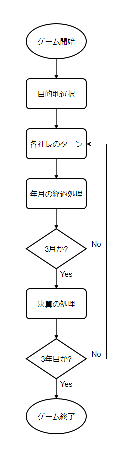
\includegraphics[scale=2.3]{processgame.eps}
        \caption{ゲームの進行}
         \label{processgame}
        \end{figure}

    \subsection{マップの設定}
    マップの設定について説明する.図\ref{map}に本ゲームのマップを示す.図\ref{map}の地名からも読み取れるように,本ゲームは長野県を舞台にしている.
    ただし,実際のゲームでは駅名は表示されない仕様になっている.マップは32$\times$32の画像を敷き詰める形で描画しており,サイズは960$\times$960である.
    なお,ウィンドウサイズは幅480,高さ320のため実際のゲームでは,行動中の社長を中心として画面におさまる部分だけを描画している.

    \begin{figure}[H]
        \centering
        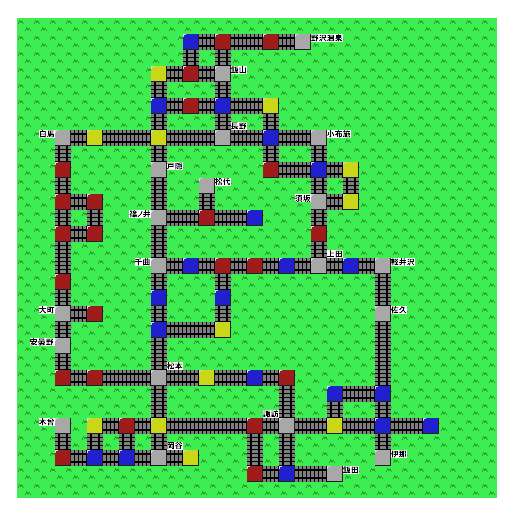
\includegraphics[scale=1.9]{map.eps}
        \caption{ゲームのマップ}
         \label{map}
        \end{figure}

    マップを描画する画像には表\ref{mapimage}に示す種類のものがある.
    これらの画像は「/mapparts」に保存されている.背景は季節によって変化する.月と季節は次に示すようになっている.図\ref{map}の
    マップは背景が春の場合である.季節ごとに背景が変化する仕様は桃鉄を参考にした.
    \begin{itemize}
        \item 春 : 3月~5月 
        \item 夏 : 6月~8月 
        \item 秋 : 9月~11月 
        \item 冬 : 12月~2月 
      \end{itemize}

\begin{table}[H]
  \caption{マップとして描画される画像の種類}
\label{mapimage}
\begin{center}
    \begin{tabular}{c|c|c}\hline
        画像の意味 & 画像のファイル名 & 実際の色や模様 \\ \hline \hline
        背景(春) & season1.png & 明るい緑 \\ 
        背景(夏) & season2.png & 濃い緑 \\
        背景(秋) & season3.png & 茶色 \\
        背景(冬) & season4.png & 白 \\
        プラス駅 & map1.png & 青 \\
        マイナス駅 & map2.png & 赤 \\
        カード駅 & map3.png & 黄色 \\
        物件駅 & map4.png & 灰色 \\ 
        線路(縦) & map5.png & 灰色背景に黒の線路 \\ 
        線路(横) & map6.png & 灰色背景に黒の線路 \\ 
        目的地駅 & map7.png & 灰色背景に駅のマーク\\ \hline
    \end{tabular}
\end{center}
\end{table}

    \subsection{駅の設定}
    駅の設定について説明する.サイコロをふって移動した社長が停車できる駅の種類には,表\ref{mapimage}に示したように,「プラス駅」,「マイナス駅」,「カード駅」,「物件駅」,「目的地駅」の5つがある.
    プラス駅は停車するとお金がもらえる駅である.もらえるお金は夏が最も多く,冬が最も少ない仕様になっている.マイナス駅は停車すると所持金が減少する駅である.
    減少する金額は夏が最も少なく,冬が最も多い仕様になっている.減少する額によっては所持金が負になる,いわゆる借金という状態になることがある.この場合,
    物件を売却することで借金を返済する処理が行われる.本ゲームでの借金の返済は売却する物件を選択する方式ではなく,自動で売却する物件を選ぶ方式を採用した.
    売却する物件の優先順位は次に示す通りである.なお,所持している全ての物件を売却しても借金が返済できない場合は所持金が負となった状態でターンが終了する.
    \begin{enumerate}
        \item 独占している駅の物件でなく,借金額よりも価格が高い物件
        \item 独占している駅の物件でなく,借金額よりも価格が低い物件
        \item 独占している物件で,借金額よりも価格が高い物件
        \item 独占している物件で,借金額よりも価格が低い物件
    \end{enumerate}
     カード駅は停車するとカードがもらえる駅である.カードは5枚まで所持することができ,カード駅に停車したときに既に5枚カードを持っている場合,この処理はスキップされる.
    カードは表\ref{cardlist}に示す8種類がある.カード名は桃鉄を参考にした.表\ref{cardlist}のカードのうち,急行カード,特急カード,新幹線カードの3種類は
    カードを仕様したあとにサイコロをふって移動することができる.他のカードについは,成功,失敗にかかわらずターンが終了する.
    \begin{table}[H]
        \caption{カード名と効果}
      \label{cardlist}
      \begin{center}
          \begin{tabular}{c|c}\hline
              カード名 & カードの効果 \\ \hline \hline
              急行カード & サイコロが2個に増える.\\
              特急カード & サイコロが3個に増える.\\
              新幹線カード & サイコロが4個に増える.\\
              サミットカード & すべての社長を自分のマスに集める.3分の2の確率で成功する.\\
              ぶっとびカード & ランダムな物件駅に移動する. \\
              10億円カード & 10億円が手に入る.\\
              徳政令カード & 借金を負っている社長の所持金が0円になる.\\
              剛速球カード & 他の社長のカードをすべて破棄する.2分の1の確率で成功する.\\ \hline
          \end{tabular}
      \end{center}
      \end{table}

      \subsection{決算の処理}
      決算の処理について説明する.決算は3月が終了すると行われる処理である.決算は,所持している物件に応じて各社長の所持金が
      増加する処理である.ある社長が決算で得られる金額$S$を計算する方法について説明する.物件を$n$個持っており,所持している$i$番目の物件の価格$p_i$,
      収益率$r_i$,その物件が所属する駅が自分の独占のとき$d_i=2$,独占でないとき$d_i=1$とする.このとき,決算で得られる金額$S$は式(\ref{kessan})で表せる.
      \begin{equation}
        S = \sum_{i=1}^{n} \frac{p_i r_i d_i}{100}
        \label{kessan}
      \end{equation}
      例えば,ある社長が,図\ref{bukkenex}の「やわたやいそごろう」と「アイススケートじょう」を所持している場合に
      決算でもらえる金額を計算してみる.式(\ref{kessan})に値を代入して計算を行うと,式(\ref{kessan_ex1})に示すように1800万円になる.
      この例では独占はしていないから$d_i$は常に1である.

      \begin{eqnarray}
        S &=& \sum_{i=1}^{n} \frac{p_i r_i d_i}{100} \\
          &=& \frac{1}{100} \left( 6000\times10^4 \cdot 20 + 20000\times10^4 \cdot 3 \right) \\
          &=& 1800 \times10^4
        \label{kessan_ex1}
      \end{eqnarray}    
       本ゲームは3年決戦であるため,3年目の決算は「最終成績」という形で表示される.最終成績を表示した後はゲームを終了するように促す画面を表示する.
    
      \section{実行環境とビルド方法}
      本章では,実行環境,ビルド方法,ディレクトリ構造の3つについて述べる.
      \subsection{実行環境}
      実行環境を\ref{env}に示す.gccとは「GNU Compiler Collection」の略称で,GNUプロジェクトが公開しているコンパイラのことである.
      makeはMakefileにプログラムのコンパイルやリンクの方法を指示することで,コンパイルを簡単に行うことができるツールのことである.
      makeを用いることは,gccコンパイル時に,長いオプションを入力しなくてよい,ファイルの更新を取得して必要なものだけをコンパイルしてくれる
      という利点がある.
      
      \begin{table}[H]
        \caption{実行環境}
      \label{env}
      \begin{center}
          \begin{tabular}{c|l}\hline
            CPU & Intel(R) Core(TM) i7-6500U 2.50GHz  \\ 
            メモリ & 16.0GB DDR4 \\
            OS & Microsoft Windows 10 Home \\
            gcc &  version 9.3.0 \\
            make & version 4.3 \\ \hline
          \end{tabular}
      \end{center}
      \end{table}
      
      \subsection{ビルド方法}
      ビルド方法について説明する.まず,「j17406.tar.gz」を保存したディレクトリに移動する.次にリスト\ref{kaito}に示すコマンドを実行する.
      リスト\ref{kaito}のコマンドを実行することで,j17406.tar.gzが解凍される.
      \begin{lstlisting}[basicstyle=\ttfamily\footnotesize, frame=single,label=kaito,caption=j17406.tar.gzの解凍]
gzip -dv j17406.tar.gz
tar xvf j17406.tar
        \end{lstlisting}
        解凍を行えたから,リスト\ref{make}の1行目のコマンドを実行してビルドを行う.リスト\ref{make}のコマンドを実行して
        「j17406.exe」が生成されていればビルド成功である.「j17406.exe」の実行はリスト\ref{make}の2行目のコマンドで行う.
        リスト\ref{make}の2行目のコマンドを実行して図\ref{sp4}に示す画面が表示されれば,ゲームの起動が成功している.
        \begin{lstlisting}[basicstyle=\ttfamily\footnotesize, frame=single,label=make,caption=makeコマンド]
make
.\j17406.exe
        \end{lstlisting}  

    \begin{figure}[H]
        \centering
        \includegraphics[scale=1.8]{sp4.png}
        \caption{ゲームのスタート画面}
         \label{sp4}
        \end{figure}

      \subsection{ディレクトリ構造}
      リスト\ref{tree}に「/j17406」のディレクトリ構造を示す.リスト\ref{tree}はtreeコマンドを用いてディレクトリ構造を
      表示したものである.ここでは,深さ1のファイル,ディレクトリのみを表示している.なぜなら,日本語画像や物件情報を保存しているディレクトリがあるため全てのファイルを
      表示すると見にくくなってしまうからである.
      ゲームの実装のためのコードは「game.c」および「j17406.c」に記述している.また,関数,定数の定義は
      「game.h」に記述している.画像は,画像の種類ごとにディレクトリを分けて保存している.ディレクトリ名と保存している画像の種類は
      表\ref{imgdir}の通りである.property.txtおよび「/property」に保存されているtxtファイルは駅の情報および物件の情報を保存している.
    
        \begin{lstlisting}[basicstyle=\ttfamily\footnotesize, frame=single,label=tree,caption=ディレクトリ構造]
j17406
├── Makefile
├── charimg
├── description.html
├── descriptionimg
├── dice
├── eventparts
├── game.c
├── game.h
├── icon.o
├── j17406.c
├── mapparts
├── property
├── property.txt
└── readme.txt
        \end{lstlisting}    
        
      \begin{table}[H]
        \caption{画像を保存するディレクトリ}
      \label{imgdir}
      \begin{center}
          \begin{tabular}{c|c}\hline
            ディレクトリ名 & 保存している画像の種類 \\ \hline \hline
            charimg & 日本語を画面に表示するための画像 \\
            dice & サイコロの画像 \\ 
            eventparts & 社長の画像,スタート画面,決算,ゲーム終了画面 \\ 
            mapparts & マップ描画のための画像 \\
            descriptionimg & description.htmlのための画像 \\ \hline
          \end{tabular}
      \end{center}
      \end{table}
        
    
    \section{プログラムの説明と実行結果}
    本章では次に示すプログラムの説明および実行結果について述べる.なお,プログラム中に登場する定数の値は付録の
    「game.h」(リスト!)を参照してほしい.
    \begin{enumerate}
        \item playerstatus構造体
        \item propertystatus構造体
        \item stationstatus構造体
        \item Map配列の定義
        \item 日本語プロトコルの定義
        \item 画像の読み込み
        \item 画像および日本語の表示
        \item 駅および物件情報の読み込み
        \item メイン関数(j17406.c)
        \item 画面サイズ変更への対応(Reshape関数)
        \item ゲームの進行状況管理
        \item ゲームの初期化とタイトル画面の表示
        \item 目的地の設定処理
        \item プレイヤーおよびマップの描画処理
        \item ターンのはじめの処理
        \item サイコロをふる処理
        \item マス移動および停車駅の判定処理
        \item 物件駅の処理
        \item プラス駅の処理
        \item マイナス駅および借金の処理
        \item カード駅の処理
        \item ターン終了時の処理
        \item 決算および最終成績の処理
        \item カードを使用したときの処理
    \end{enumerate}    

    \subsection{playerstatus構造体}
    playerstatus構造体の定義と初期化について説明する.まず,playerstatus構造体の定義について説明する.
    playerstatus構造体は一人の社長の情報を保持するための構造体である.リスト\ref{playerstatus}に「game.h」におけるplayerstatus構造体の
    定義を示す. playerstatus構造体は「社長名」,「所持金」,「総資産」,「現在の座標(x,y)」,「カード枚数」,「カードの通し番号」の7つをメンバとして持っている.
    所持金および総資産は万円単位で扱うものとする.例えば所持金が「2200万円」場合,メンバmoneyには2200が代入される.これ以降にも金額を
    扱うための変数が登場するが,そのすべての変数は万円単位で扱うものとする.
    また,11行目のようにplayerstatus構造体の配列を定義することで,プレイ人数3人分の情報を保持する構造体の配列を作成している.
    \begin{lstlisting}[basicstyle=\ttfamily\footnotesize, frame=single,label=playerstatus,caption=playerstatus構造体の定義と初期化]
// プレイヤーの情報構造体
struct playerstatus{
    char name[NAMEMAX]; // プレイヤー名
    int money; // 所持金
    int assets; // 総資産
    int x; // x座標(実描画座標)
    int y; // y座標(実描画座標)
    int cardnum; // 持っているカード枚数
    int card[CARDMAX]; // カードの番号記憶
};
    
    typedef struct playerstatus player;
    player players[PLAYERNUM]; // 人数分の配列を確保
    \end{lstlisting}

    次にplayerstatus構造体を初期化する関数について説明する.リスト\ref{InitPlayer}に,playerstatus構造体を初期化する関数である
    InitPlayer関数のコードを示す.InitPlayer関数の内部では,for文を用いてplayerstatus構造体の配列を初期化している.
    リスト\ref{InitPlayer}中の定数の値はINITXが224(7$\times$32),INITYが160(5$\times$32),INITMONEYは10000である.
    メンバ(x,y)に代入している値は,!
    \begin{lstlisting}[basicstyle=\ttfamily\footnotesize, frame=single,label=InitPlayer,caption=InitPlayer関数]
// プレイヤー構造体を初期化
void InitPlayer(void){
    int i,j;
    for(i=0;i<PLAYERNUM;i++){
        //プレイヤーhoge
        sprintf(players[i].name,"llpureiiyallms%d",i+1);
        players[i].x=INITX;
        players[i].y=INITY;
        players[i].money=INITMONEY;
        players[i].assets=0;
        players[i].cardnum=0;
        for(j=0;j<CARDMAX;j++){
            players[i].card[j]=0;
        }
    }
}
            \end{lstlisting}

    \subsection{propertystatus構造体}
    propertystatus構造体は一つの物件の情報を保持するための構造体である.「game.h」におけるpropertystatus構造体の定義をリスト\ref{propertystatus}に示す.
    propertystatus構造体は「物件名」,「物件保持者」,「価格」,「収益率」の4つをメンバとして持っている.物件保持者は表\ref{whohold}のルールで扱うものとする.
   \begin{lstlisting}[basicstyle=\ttfamily\footnotesize, frame=single,label=propertystatus,caption=propertystatus構造体の定義]
   // 物件情報構造体
   struct propertystatus{
   char name[STRMAX]; // 物件名
   int holder; // 物件所持者
   int price; // 価格
   int earnings; // 収益率
   };
   
   typedef struct propertystatus property;
   \end{lstlisting}
   
   \begin{table}[H]
     \caption{物件保持者メンバの意味}
   \label{whohold}
   \begin{center}
       \begin{tabular}{c|c}\hline
       値 & 保持者 \\ \hline \hline
         0 & 保持者なし \\
         1 & 社長1 \\
         2 & 社長2 \\
         3 & 社長3 \\ \hline
       \end{tabular}
   \end{center}
   \end{table}

    \subsection{stationstatus構造体}
stationstatus構造体は一つの駅の情報を保持するための構造体である.リスト\ref{stationstatus}にstationstatus構造体の定義を示す.
stationstatus構造体は,「駅名」,「駅の座標(x,y)」,「独占フラグ」,「物件の数」,「propertystatus構造体の配列」の6つをメンバとして持つ.
駅の座標(x,y)はplayerstatus構造体のような実座標ではなく,マップを描画するための配列のインデックスである.独占フラグは
その駅を誰が独占しているかを判別するために用いる.独占フラグの値とその意味は表\ref{whohold}と同じである.
\begin{lstlisting}[basicstyle=\ttfamily\footnotesize, frame=single,label=stationstatus,caption=stationstatus構造体の定義と初期化]
// 駅情報構造体
struct stationstatus{
char name[STRMAX]; // 駅名
int x; // x座標
int y; // y座標
int ismonopoly; // 独占フラグ
int propertynum; // 物件数
property plist[PROPERTMAX]; // 物件情報構造体の配列
};

typedef struct stationstatus station;
station stations[STATIONNUM]; // 駅の数分の配列を確保
station distination; // 目的地配列
\end{lstlisting}

    \subsection{Map配列の定義}
    マップの情報はMap配列が保持している.Map配列の定義をリスト\ref{Maparray}に示す.
    マップのサイズは30$\times$30で,配列のサイズは30$\times$31である.
    x方向の配列のサイズが1大きいのは,null文字を格納するためである.Map配列の文字列は
    「A」,「B」,「C」,「P」,「M」,「-」,「\textbar」のいずれかの文字から構成されている.表\ref{mapstr}に
    文字と実際に表示される画像の関係を示す.
    \begin{lstlisting}[basicstyle=\ttfamily\footnotesize, frame=single,label=Maparray,caption=Map配列の定義]
// マップ配列
char Map[YMAX][XMAX+1] = { //NULL文字に気を付ける
       //012345678901234567890123456789      
        "AAAAAAAAAAAAAAAAAAAAAAAAAAAAAA", // 0
        "AAAAAAAAAAAP-M--M-BAAAAAAAAAAA", // 1
        "AAAAAAAAAAA|A|AAAAAAAAAAAAAAAA", // 2
        "AAAAAAAAAC-M-BAAAAAAAAAAAAAAAA", // 3
        "AAAAAAAAA|AAA|AAAAAAAAAAAAAAAA", // 4
        "AAAAAAAAAP-M-P--CAAAAAAAAAAAAA", // 5
        "AAAAAAAAA|AAA|AA|AAAAAAAAAAAAA", // 6
        "AAAB-C---C---B--P--BAAAAAAAAAA", // 7
        "AAA|AAAAA|AAAAAA|AA|AAAAAAAAAA", // 8
        "AAAMAAAAABAAAAAAM--P-CAAAAAAAA", // 9
        "AAA|AAAAA|AABAAAAAA|A|AAAAAAAA", // 0
        "AAAM-MAAA|AA|AAAAAAB-CAAAAAAAA", // 1
        "AAA|A|AAAB--M--PAAA|AAAAAAAAAA", // 2
        "AAAM-MAAA|AAAAAAAAAMAAAAAAAAAA", // 3
        "AAA|AAAAA|AAAAAAAAA|AAAAAAAAAA", // 4
        "AAA|AAAAAB-P-M-M-P-B-P-BAAAAAA", // 5
        "AAAMAAAAA|AAA|AAAAAAAAA|AAAAAA", // 6
        "AAA|AAAAAPAAAPAAAAAAAAA|AAAAAA", // 7
        "AAAB-MAAA|AAA|AAAAAAAAABAAAAAA", // 8
        "AAA|AAAAAP---CAAAAAAAAA|AAAAAA", // 9
        "AAABAAAAA|AAAAAAAAAAAAA|AAAAAA", // 0
        "AAA|AAAAA|AAAAAAAAAAAAA|AAAAAA", // 1
        "AAAM-M---B--C--P-MAAAAA|AAAAAA", // 2
        "AAAAAAAAA|AAAAAAA|AAP--PAAAAAA", // 3
        "AAAAAAAAA|AAAAAAA|AA|AA|AAAAAA", // 4
        "AAABAC-M-C-----M-B--C--P--PAAA", // 5
        "AAA|A|A|A|AAAAA|A|AAAAA|AAAAAA", // 6
        "AAAM-P-P-B-CAAA|A|AAAAABAAAAAA", // 7
        "AAAAAAAAAAAAAAAM-P--BAAAAAAAAA", // 8
        "AAAAAAAAAAAAAAAAAAAAAAAAAAAAAA"  // 9
};
    \end{lstlisting}

    \begin{table}[H]
        \caption{文字と画像の対応}
      \label{mapstr}
      \begin{center}
          \begin{tabular}{c|c}\hline
            文字 & 表示される画像 \\ \hline \hline
            A & 背景 \\ 
            B & 物件駅 \\ 
            C & カード駅 \\ 
            P & プラス駅 \\ 
            M & マイナス駅 \\ 
            - & 線路(横) \\ 
            \textbar  & 線路(縦) \\ \hline
          \end{tabular}
      \end{center}
      \end{table}

    \subsection{日本語プロトコルの定義}
    桃鉄をイメージしたゲームを実装するうえで,日本語を画面に表示できなければ,ローマ字が並んでわかりにくい.しかしGLUTは日本語に対応していない.
そこで画像を用いて日本語をゲーム画面に描画する機能を作成した.これを日本語プロトコルと呼ぶことにする.文字色は黒と赤のどちらかで描画することが可能である.
作成した日本語プロトコルでは次に示す文字を画面に表示することができる.一部のアルファベット,記号,漢字をまとめて特殊文字と呼ぶことにする.
\begin{itemize}
  \item 50音(ひらがな,カタカナ)
  \item 濁音(ひらがな,カタカナ)
  \item 半濁音(ひらがな,カタカナ)
  \item 小文字(っ,ゃ,ゅ,ょ)(ひらがな,カタカナ)
  \item 数字
  \item 一部のアルファベット(W,A,S,D,E,Q)
  \item 一部の記号(読点,句点,\%,マイナスの記号(-),プラスの記号(+))
  \item ゲームに頻出する漢字(億,万,円)
\end{itemize}

これらの画像は「/charimg」に保存されている.画像のサイズはすべて32$\times$32pxである.画像名の意味は図\ref{howname}の通りである.
どの文字か判別する2文字はコード中で日本語を表示するための文字列に対応している.実際の文字と日本語プロトコルにおける文字の表現
方法は表\ref{jpp}の通りである.改行およびスペースは画像にはないが,画像を表示する位置を調整することで表現できる.表\ref{jpp}の情報は
game.cでリスト\ref{jpProtcolarray}に示すように定義されている.

\begin{figure}[H]
  \centering
  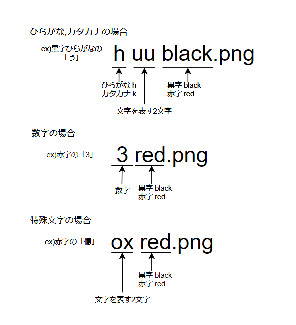
\includegraphics[scale=1.7]{howname.eps}
  \caption{画像の名前の意味}
   \label{howname}
  \end{figure}    

  \begin{table}[H]
    \caption{日本語プロトコルの文字表現}
  \label{jpp}
  \begin{center}
      \begin{tabular}{c|c|c|c|c}\hline
あ aa & い ii & う uu & え ee & お oo \\ 
か ka & き ki & く ku & け ke & こ ko \\ 
さ sa & し si & す su & せ se & そ so \\ 
た ta & ち ti & つ tu & て te & と to \\ 
な na & に ni & ぬ nu & ね ne & の no \\ 
は ha & ひ hi & ふ hu & へ he & ほ ho \\ 
ま ma & み mi & む mu & め me & も mo \\ 
や ya & -  & ゆ yu & -  & よ yo \\ 
ら ra & り ri & る ru & れ re & ろ ro \\ 
わ wa & -  & を wo & -  & ん nn \\ 
ゃ la & - & ゅ lu & っ lt & ょ lo \\ 
が ga & ぎ gi & ぐ gu & げ ge & ご go \\ 
ざ za & じ zi & ず zu & ぜ ze & ぞ zo \\
だ da & ぢ di & づ du & で de & ど do \\
ば ba & び bi & ぶ bu & べ be & ぼ bo \\ 
ぱ pa & ぴ pi & ぷpu &  ぺ pe & ぽ po \\ 
0  0 & 1  1 & 2  2 & 3  3 & 4  4 \\ 
5  5 & 6  6 & 7  7 & 8  8 & 9  9 \\ 
円 ex & 万 mx & 億 ox & \% px & - ms \\ 
+ ps & 句点 mr & 読点 tn & Q xq & W xw \\ 
E xe & A xa & S xs & D xd & - \\ 
改行 xx & スペース ss & - & - & - \\ \hline
      \end{tabular}
  \end{center}
  \end{table}
  
  \begin{lstlisting}[basicstyle=\ttfamily\footnotesize, frame=single,label=jpProtcolarray,caption=jpProtcol配列]
// 日本語プロトコル
char jpProtcol[JPMAX+SPMAX][3] = {"aa","ii","uu","ee","oo",
                        "ka","ki","ku","ke","ko",
                        "sa","si","su","se","so",
                        "ta","ti","tu","te","to",
                        "na","ni","nu","ne","no",
                        "ha","hi","hu","he","ho",
                        "ma","mi","mu","me","mo",
                        "ya","yu","yo",
                        "ra","ri","ru","re","ro",
                        "wa","wo","nn",
                        "lt","la","lu","lo",
                        "ga","gi","gu","ge","go",
                        "za","zi","zu","ze","zo",
                        "da","di","du","de","do",
                        "ba","bi","bu","be","bo",
                        "pa","pi","pu","pe","po",
                        "0","1","2","3","4","5"
                        ,"6","7","8","9",
                        "ex","mx","ox","px","ms","ps",
                        "mr","tn","xq","xw","xe","xa","xs","xd"
                        };

  \end{lstlisting} 
  
  \subsection{画像の読み込み}
  画像を読み込む方法について説明する.リスト\ref{readImg}に画像を読み込むためのreadImg関数のコードを示す.
  処理の内容はファイル名や読み込み先を変えて画像を読み込んでいるだけだから,リスト\ref{readImg}の7行目から11行目のイベントマップの読み込みを
  例に説明する.画像を読み込むためには2つの変数が必要である.今の例ではspimgとspinfoである.変数spimgには読み込んだ画像を識別するための値が
  代入され,変数spinfoには読み込んだ画像のと横幅,縦幅を代表とする情報が格納される.これらの変数にpngBind関数を用いて読み込んだ画像の
  情報を与えることで画像の読み込みを行っている.
  \begin{lstlisting}[basicstyle=\ttfamily\footnotesize, frame=single,label=readImg,caption=readImg関数]
// 画像読み込み
void readImg(void){
    int i;
    char fname[100];

    // イベントマップ読み込み
    for(i=0;i<SP_NUM;i++){
        sprintf(fname,".\\eventparts\\sp%d.png",i+1);
        spimg[i] = pngBind(fname, PNG_NOMIPMAP, PNG_ALPHA, 
       &spinfo[i], GL_CLAMP, GL_NEAREST, GL_NEAREST);        
    }

   // 季節マップ読み込み 
    for(i=0;i<SEASON_NUM;i++){
        sprintf(fname,".\\mapparts\\season%d.png",i+1);
        seasonimg[i] = pngBind(fname, PNG_NOMIPMAP, PNG_ALPHA, 
       &seasoninfo[i], GL_CLAMP, GL_NEAREST, GL_NEAREST);        
    }

    // マップイメージ読み込み
    for(i=0;i<=MAP_NUM;i++){
        sprintf(fname,".\\mapparts\\map%d.png",i+1);
        mapimg[i] = pngBind(fname, PNG_NOMIPMAP, PNG_ALPHA, 
       &mapinfo[i], GL_CLAMP, GL_NEAREST, GL_NEAREST);
    }
    // プレイヤー画像を読み込み
    for(i=0;i<PLAYERNUM;i++){
        sprintf(fname,".\\eventparts\\player%d.png",i+1);
        playerimg[i] = pngBind(fname, PNG_NOMIPMAP, PNG_ALPHA, 
       &playerinfo[i], GL_CLAMP, GL_NEAREST, GL_NEAREST);
    }

    // サイコロの画像を読み込み
    for(i=0;i<DICEMAX;i++){
        sprintf(fname,".\\dice\\dice%d.png",i+1);
        diceimg[i] = pngBind(fname, PNG_NOMIPMAP, PNG_ALPHA, 
       &diceinfo[i], GL_CLAMP, GL_NEAREST, GL_NEAREST);
    }
    // read Hiragana black
    for(i=0;i<JPMAX;i++){
        sprintf(fname,".\\charimg\\h%sblack.png",jpProtcol[i]);
        hblackimg[i] = pngBind(fname, PNG_NOMIPMAP, PNG_ALPHA, 
        &hblackinfo[i], GL_CLAMP, GL_NEAREST, GL_NEAREST);
    }

    // read Hiragana red
    for(i=0;i<JPMAX;i++){
        sprintf(fname,".\\charimg\\h%sred.png",jpProtcol[i]);
        hredimg[i] = pngBind(fname, PNG_NOMIPMAP, PNG_ALPHA, 
        &hredinfo[i], GL_CLAMP, GL_NEAREST, GL_NEAREST);
    }
    // read Katakana black
    for(i=0;i<JPMAX;i++){
        sprintf(fname,".\\charimg\\k%sblack.png",jpProtcol[i]);
        kblackimg[i] = pngBind(fname, PNG_NOMIPMAP, PNG_ALPHA, 
        &kblackinfo[i], GL_CLAMP, GL_NEAREST, GL_NEAREST);
    }
    // read Katakana red
    for(i=0;i<JPMAX;i++){
        sprintf(fname,".\\charimg\\k%sred.png",jpProtcol[i]);
        kredimg[i] = pngBind(fname, PNG_NOMIPMAP, PNG_ALPHA, 
        &kredinfo[i], GL_CLAMP, GL_NEAREST, GL_NEAREST);
    }
    // read Special Str red
    for(i=JPMAX;i<JPMAX+SPMAX;i++){
        sprintf(fname,".\\charimg\\%sred.png",jpProtcol[i]);
        hredimg[i] = pngBind(fname, PNG_NOMIPMAP, PNG_ALPHA, 
        &hredinfo[i], GL_CLAMP, GL_NEAREST, GL_NEAREST);
    }
    // read Special Str black
    for(i=JPMAX;i<JPMAX+SPMAX;i++){
        sprintf(fname,".\\charimg\\%sblack.png",jpProtcol[i]);
        hblackimg[i] = pngBind(fname, PNG_NOMIPMAP, PNG_ALPHA, 
        &hblackinfo[i], GL_CLAMP, GL_NEAREST, GL_NEAREST);
    }
}
      \end{lstlisting} 
  \subsection{画像および日本語の表示}  
  画像および日本語をゲーム画面に表示する方法について説明する.まず,画像を表示する方法について説明する.画像の表示
  はリスト\ref{PutSprite}に示すPutSprite関数を用いて行っている.PutSprite関数は「Springs of C」!から引用した関数である.
  リスト\ref{PutSprite}のコードでは,引用した関数に,引数として画像の表示倍率scaleを加え,画像の縮小を行えるようにした.
  画像の表示倍率はリスト\ref{PutSprite}の6行目および7行目でテクスチャの幅と高さをscale倍することで行っている.
  \begin{lstlisting}[basicstyle=\ttfamily\footnotesize, frame=single,label=PutSprite,caption=PutSprite関数]
// (x,y)に大きさscaleの画像を表示
void PutSprite(int num, int x, int y, pngInfo *info,double scale)
{
    int w, h;  //  テクスチャの幅と高さ

    w = info->Width*scale;   //  テクスチャの幅と高さを取得する
    h = info->Height*scale;

    glPushMatrix();
    glEnable(GL_TEXTURE_2D);
    glBindTexture(GL_TEXTURE_2D, num);
    glColor4ub(255, 255, 255, 255);

    glBegin(GL_QUADS);  //  幅w, 高さhの四角形

    glTexCoord2i(0, 0); 
    glVertex2i(x, y);

    glTexCoord2i(0, 1);
    glVertex2i(x, y + h);

    glTexCoord2i(1, 1);
    glVertex2i(x + w, y + h);

    glTexCoord2i(1, 0);
    glVertex2i(x + w, y);

    glEnd();

    glDisable(GL_TEXTURE_2D);
    glPopMatrix();
}
          \end{lstlisting} 

    次に日本語の表示方法について説明する.リスト\ref{jpfunc}に日本語を表示するための関数であるdrawChar関数および
    drawString関数のコードを示す.drawChar関数は「1文字」の日本語を表示する関数であり,drawString関数はdrawChar関数を
    連続して呼び出して文字列を表示する関数である.drawChar関数は引数としてjpProtcol配列(リスト\ref{jpProtcolarray})の
    インデックスnum,ひらがな/カタカナのどちらで表示するかを示すkh,黒/赤のどちらで描画するかを示すcolor,描画する実座標(x,y),
    表示倍率scaleの6つを受け取る.引数khは0のときひらがな,1のときカタカナである.引数colorは0のとき黒,1のとき赤である.
    drawChar関数の内部では,受け取った引数から表示する文字の種類を判断し,PutSprite関数で描画する処理を行っている.\\
     drawString関数は引数として描画する文字列string,文字色color,実座標(x,y),表示倍率scaleの5つを受け取る.drawString関数
    の内部では,まず引数として受け取った文字列stringを1文字または2文字ずつ取り出して,文字の種類を判断している.リスト\ref{jpfunc}では,
    29行目および30行目が数字かどうかの判別を行っている部分である.日本語の判別は35行目,特殊文字は41行目で判定している.例外として
    ひらがな/カタカナ切り替えは47行目,改行は51行目で判定している.空白は判定していないが,これは該当する文字がない場合に何も
    描画せずに文字を表示する位置がずれることを利用している.このため,空白は「ss」以外の文字列でも表現できるがコードのわかり
    やすさという観点から「ss」という文字に統一している.文字の種類の判断が行えたら,jpProtcol配列におけるその文字のインデックス
    および描画のための情報をdrawChar関数に渡して描画を行っている.最後に58行目から63行目で次に表示する文字の位置を計算する処理
    を行っている.これらの処理によって画面に日本語を描画している.

    \begin{lstlisting}[basicstyle=\ttfamily\footnotesize, frame=single,label=jpfunc,caption=日本語表示のための関数]
// 1文字の日本語を表示
// int kh : 0,Hiragana 1,Katakana
// int color 0,black 1,red
void drawChar(int num,int kh,int color,int x,int y,double scale){
    if(kh==0){
        if(color==0){ // hiragana black
            PutSprite(hblackimg[num], x, y, &hblackinfo[num],scale);
        }else{ //hiragana red
            PutSprite(hredimg[num], x, y, &hredinfo[num],scale);
            }
        }else{ 
        if(color==0){ // katakana black
            PutSprite(kblackimg[num], x, y, &kblackinfo[num],scale);
        }else{ // katakana red
            PutSprite(kredimg[num], x, y, &kredinfo[num],scale);
        }
    }
}

// 引数stringの文字列を表示
void drawString(char *string,int color,int xo,int yo,double scale){
    int i,j;
    int len = strlen(string);
    int x=xo;
    int y=yo;
    int flg;
    int kh=0;
    for(i=0;i<len;i++){
        flg=string[i]-'0'; // インデクス計算
        if((flg>=0)&&(flg<=9)){ // 数字描画
            drawChar(JPMAX+flg,0,color,x,y,scale);
            flg=1;
        }else{
            for(j=0;j<JPMAX;j++){ //日本語描画
                if((jpProtcol[j][0]==string[i])&&(jpProtcol[j][1]==string[i+1])){
                    drawChar(j,kh,color,x,y,scale);
                    break;
                }
            }       
            for(j=JPMAX+10;j<JPMAX+SPMAX;j++){ //特殊文字描画
                if((jpProtcol[j][0]==string[i])&&(jpProtcol[j][1]==string[i+1])){
                    drawChar(j,kh,color,x,y,scale);
                    break;
                }
            }
            flg=1;
            if((string[i]=='l')&&(string[i+1]=='l')){ //ひらがな/カタカナ切り替え
                kh=1-kh;
                flg=0;
            }
            if((string[i]=='x')&&(string[i+1]=='x')){ // 改行
                x=xo;
                flg=0;
                y+=IMGSIZE*scale;
            }     
            i++;
        }
        if(flg==1){ // 次の座標に移動
            x+=IMGSIZE*scale;
            if(x>InitWidth-22){
                x=xo;
                y+=IMGSIZE*scale;
            }
        }
    }
}

                  \end{lstlisting} 
  \subsection{駅および物件情報の読み込み}
  駅および物件の情報を読み込む方法について説明する.動作確認は次節のメイン関数で行う.まず,駅の情報を読み込む方法について説明する.
  駅の情報はproperty.txtに保存されている.リスト\ref{propertytxt}にproperty.txtの内容を示す. property.txt
  は「駅名 x座標,y座標」という形式ですべての駅の情報が保存されている.駅名は日本語プロトコルにおける
  駅名の表示である.座標は実座標ではなく, Map配列(リスト\ref{Maparray})のインデックスである.
  例えば飯山駅の場合,駅名が「iiiiyama」, Map配列における座標が(13,3)になっている.リスト\ref{Maparray}の(13,3)を確認すると
  「B」つまり物件駅になっている.また,図\ref{map}からこの位置にある駅は飯山駅であることがわかる.これらよりproperty.txtで
  定義した駅名および座標が,Map配列や画面表示と合致していることが確認できた.同様にして全ての駅について
  駅名と座標が間違っていないことを筆者は確認した.
\begin{lstlisting}[basicstyle=\ttfamily\footnotesize, frame=single,label=propertytxt,caption=property.txt]
nozawaoonnsenn 18,1
iiiiyama 13,3
togakusi 9,9
nagano 13,7
oobuse 19,7
suzaka 19,11
matusiro 12,10
sinonoii 9,12
hakuba 3,7
oooomati 3,18
tikuma 9,15
uueeda 19,15
karuiizawa 23,15
aadumino 3,20
saku 23,18
matumoto 9,22
suwa 17,25
kiso 3,25
ookaya 9,27
iiiida 20,28
iina 23,27
        \end{lstlisting}   
    
    property.txtの形式が確認できたから,これを読み込む関数について説明する.リスト\ref{readStation}に駅の情報を読み込むための関数
    であるreadStation関数のコードを示す.リスト\ref{readStation}においてファイルから読み取った情報をstationstatus構造体に代入しているのは
    11行目から14行目である.11行目でfscanf関数を用いて「駅名 x座標,y座標」という情報を構造体に代入している.
\begin{lstlisting}[basicstyle=\ttfamily\footnotesize, frame=single,label=readStation,caption=readStation関数]
// ファイルから駅情報を取得
// stations構造体を初期化
void readStation(void){
    FILE *fp;
    int i=0;
    fp=fopen("property.txt","r");
    if(fp==NULL){ // 開けなかったとき
        printf("file not found");
        exit(0);
    }else{ // 駅名と座標を取得
        while(fscanf(fp,"%s %d,%d",stations[i].name,&stations[i].x,&stations[i].y)!=EOF){
            stations[i].ismonopoly=0; // 独占フラグ初期化
            i++;
        }
        fclose(fp);
    }
}

        \end{lstlisting}     
    
    次に物件の情報を読み込む方法について説明する.物件の情報は「/property」に「駅名.txt」という形式で保存している.
    駅名は日本語プロトコルにおける駅名である.
    リスト\ref{naganotxt}およびリスト\ref{matumototxt}に物件情報を保存しているファイルの例を示す.リスト\ref{naganotxt}は
    長野駅,リスト\ref{matumototxt}は松本駅である.物件の情報は「物件名 価格,収益率」という形式で保存している.
\begin{lstlisting}[basicstyle=\ttfamily\footnotesize, frame=single,label=naganotxt,caption=/property/nagano.txt]
rinngoeenn 600,120
rinngoeenn 600,120
yawatayaiisogorouu 6000,20 
llaaiisusukellmslltollzilouu 20000,3 
zennkouuzi 110000,30
naganokouusenn 600000,1
\end{lstlisting}  

\begin{lstlisting}[basicstyle=\ttfamily\footnotesize, frame=single,label=matumototxt,caption=/property/matumoto.txt]
giluuuniluuullpannll 1200,130 
kamikouuti 12000,80
sinnsiluuudaiigaku 60000,30
aasamaoonnsenn 80000,4
kiluuukaiitigaltkouu 90000,5
matumotozilouu 150000,5
\end{lstlisting}     

    物件情報の保存形式が確認できたから,これを読み込む関数について説明する.リスト\ref{readProperty}に
    物件の情報を読み込む関数であるreadProperty関数のコードを示す.リスト\ref{readProperty}において
    ファイルから読み取った情報をpropertystatus構造体に代入しているのは,15行目および16行目である.
    readStation関数と同様にfscanf関数を用いて「物件名 価格,収益率」という情報を構造体に代入している.
    \begin{lstlisting}[basicstyle=\ttfamily\footnotesize, frame=single,label=readProperty,caption=readProperty関数]
// ファイルから物件情報を取得
void readProperty(void){
    FILE *fp;
    int i,j;
    char fname[100];
    for(i=0;i<STATIONNUM;i++){
        sprintf(fname,".\\property\\%s.txt",stations[i].name);
        fp=fopen(fname,"r");
        j=0;
        if(fp==NULL){ // 開けなかったとき
            printf("file not found in %s",stations[i].name);
            exit(0);
        }else{
            // 物件名,値段,収益率を取得
            while(fscanf(fp,"%s %d,%d",stations[i].plist[j].name,
            &stations[i].plist[j].price,&stations[i].plist[j].earnings)!=EOF){
            stations[i].plist[j].holder=0; // 購入フラグ初期化
            j++;
        }
        stations[i].propertynum=j; // 物件数を保存
        fclose(fp);
    }

    }   
}
                \end{lstlisting}     
  \subsection{メイン関数(j17406.c)}
  
    \subsection{画面サイズ変更への対応(Reshape関数)}
    \subsection{ゲームの進行状況管理}
    \subsection{ゲームの初期化とタイトル画面の表示}
    \subsection{目的地の設定処理}
    \subsection{プレイヤーおよびマップの描画処理}
    \subsection{ターンのはじめの処理}
    \subsection{サイコロをふる処理}
    \subsection{マス移動および停車駅の判定処理}
    \subsection{物件駅の処理}
    \subsection{プラス駅の処理}
    \subsection{マイナス駅および借金の処理}
    \subsection{カード駅の処理}
    \subsection{ターン終了時の処理}
    \subsection{決算および最終成績の処理}
    \subsection{カードを使用したときの処理}
    
    \section{付録 ソースコード}

    \begin{thebibliography}{9}
        \bibitem{mmtt}  桃太郎電鉄,\url{https://www.konami.com/games/momotetsu/teiban/} ,閲覧日2021年1月5日
        \end{thebibliography}
\end{document}

